\documentclass[12pt,a4paper]{article}
\usepackage{fontspec}
\setmainfont{DejaVu Sans}
\usepackage[margin=2cm]{geometry}
\usepackage{amsmath}
\usepackage{amssymb}
\usepackage{multicol}
\usepackage[inline]{enumitem} % inline lists enabled
\usepackage{tikz}

% --- Make all math the same size as normal text (12pt) ---
\AtBeginDocument{%
  \DeclareMathSizes{12}{12}{12}{12}%
}
\everydisplay{\textstyle}

% --- One-line multiple-choice list environment ---
\newlist{choices}{enumerate*}{1}
\setlist[choices]{label=ა), itemjoin=\hspace{1.5em}, itemsep=0pt, parsep=0pt, topsep=0pt}

\begin{document}


\section*{§ 2. რაციონალური რიცხვები}
\section*{ა}

\subsection*{2.1. შეადარეთ წილადები:}

\begin{enumerate}[label=\arabic*)]
\item \( \frac{4}{11} \) და \( \frac{6}{11} \);
\item \( \frac{7}{11} \) და \( \frac{1}{4} \);
\item \( \frac{15}{19} \) და \( \frac{19}{19} \);
\item \( \frac{3}{5} \) და \( \frac{6}{8} \);
\item \( \frac{11}{12} \) და \( \frac{8}{8} \);
\item \( \frac{2}{160} \) და \( \frac{31 - 2}{240} \);
\item \( \frac{20}{35} \) და \( \frac{5}{721} \);
\item \( \frac{9}{8} \).
\end{enumerate}


\subsection*{2.2. შემდეგი რიცხვები დაალაგეთ ზრდადობის მიხედვით და მიუთითეთ მათ შორის ტოლები:}

\( \frac{1}{24}, \frac{11}{24}, \frac{12}{24}, \frac{15}{24}, \frac{16}{24}, \frac{22}{24}, \frac{3}{12}, \frac{5}{12}, \frac{3}{6}, \frac{1}{4}, \frac{2}{3}, \frac{1}{2} \)

\subsection*{2.3. განსაზღვრეთ რომელი წილადია ერთთან უფრო ახლოს და შეადარეთ ისინი:}

\( \frac{4}{3}, \frac{3}{5}, \frac{7}{8}, \frac{6}{9}, \frac{99}{100}, \frac{1010}{51231}, \frac{4}{5} \)

\subsection*{2.4.}

2 კგ შოკოლადი თანაბრად გაანაწილეს 10 პაკეტში, 5 კგ ნამცხვარი კი 15 პაკეტში. რომელი პაკეტია უფრო მძიმე?

\subsection*{2.5.}

ერთმა ტურისტმა 21 კმ გაიარა 2 სთ-ში, მეორემ კი 28 კმ 3 სთ-ში. რომელი ტურისტია უფრო სწრაფი?

\subsection*{2.6.}

გია, დათო და ბექა ღობეს ღებავდნენ. გიამ მთელი სამუშაოს \( \frac{3}{10} \) ნაწილი შეასრულა, დათომ \( \frac{5}{8} \), ბექამ კი – \( \frac{3}{40} \). რომელმა შეასრულა სამუშაოს მეტი ნაწილი?

\subsection*{2.7.}

გოგი 8 წამში 5 ნაბიჯს დგამს, ლევანი კი 5 წამში იმავე სიგრძის 3 ნაბიჯს. რომელი უფრო სწრაფად დადის?

\subsection*{2.8. მოცემული წილადი ჩაწერეთ არაწესიერი წილადის სახით:}

\( \frac{1}{2}, \frac{3}{4}, \frac{3}{5}, \frac{9}{7}, \frac{2}{1}, \frac{3}{2}, \frac{4}{3}, -\frac{2}{4}, \frac{5}{15}, \frac{6}{20}, \frac{1}{3} \).

\subsection*{2.9. მოცემული წილადი ჩაწერეთ შერეული წილადის სახით:}

\( \frac{11}{8}, \frac{12}{5} \) და სხვ.

\subsection*{2.10. შეასრულეთ მოქმედებები}

\( \frac{57}{8} + \frac{12}{61}; \frac{15}{4} - \frac{20}{11}; 3 + \frac{-5}{3}; 5 - \frac{3}{41}; \frac{100}{6} + \frac{3}{4} + 3; \frac{251}{6} + 3 + 18 + \frac{27}{30}; 7 - 20; 10 - 80 - 5;\)

\subsection*{2.11. შეასრულეთ მოქმედებები}

1) \( \frac{4}{12}; \)
2) \( 3 - 32.5; \)
3) \( 34 - 2:2; \)
4) \( \frac{43}{35}; \)
5) \( 10 - 2; \)
6) \( 3 - 9; \)
7) \( 18 : 2; \)
8) \( 7 : 11. \)

\subsection*{2.12.}

\( 1) 5,5+6,5; 2) 5,5+(-6,5); 3) -5,5+6,5; 4) -5,5+(-6,5); 5) 5,5-6,5; 6) 5,5-(-6,5); 7) -5,5-6,5; 8) -5,5-(-6,5). \)

\subsection*{2.13.}

\( 1) 2,4-3; 2) -2,4-3; 3) (-2,4)-(-3); 4) 2,4-(-3); 5) 2,4:3; 6) -2,4:3; 7) 2,4:(-3); 8) -2,4:(-3). \)

\subsection*{2.14.}

1) სპორტსმენი 2 მ სიმაღლეზე გადახტა, რაც \(1\frac{3}{7}\) ჯერ მეტია მის სიმაღლეზე. იპოვეთ სპორტსმენის სიმაღლე.

2) დილის 9 საათზე ბოძის ჩრდილის სიგრძე \(4\frac{1}{2}\) მ-ის ტოლია, რაც \(1\frac{1}{8}\)-ჯერ ნაკლებია ბოძის სიმაღლეზე. იპოვეთ ბოძის სიმაღლე.

\subsection*{2.15.}
1) \((11,81+8,19)-0,02\);
2) \(9-0,08+0,7-0,9;\)
3) \((1,11+5,19):0,21;\)
4) \((5,25-1,5):2,5.\)

\subsection*{2.16.}

1) \((7+2):3;\)
2) \((5+2)\times40;\)
3) \((5+2):100;\)
4) \((-1+1-63-96;\)
5) \((-1+3,45);\)
6) \(9 + \frac{5}{84};\)
7) \((3+2)-0,7;\)
8) \((-2-3-1)-0,4;\)
9) \( (4+3)-0,24;\)
10) \((-2+1)-4,48;\)
11) \((-4+6)-3,84.\)

\subsection*{2.17.}

სალომემ იყიდა 4,5 კგ ფორთოხალი და 1 კგ 2\(\frac{2}{5}\). რომელ ხილში გადაიხადა სალომემ მეტი და რამდენით?

\subsection*{2.18.}

\( 1) \frac{14}{5} : 2; 2) 35 : 1 - 7; 3) 39 : 20 + 4; 4) 4,4 : 1; 5) 2,8 : 7; 6) 10 : 3; 7) 65,5 : 22 - 12; 8) 32. \)

\subsection*{2.19.}

\( 1) \frac{4}{6} - \frac{2}{12} : (+2); 2) 36 : (4+3); 3) 42 : (7-3); 4) 2,2 : 2 - 3; 5) \frac{55}{4} : 15; 6) 8,8 : 30 - 10 : 35 : (+4); 7) 32. \)

\subsection*{2.20.}

ჩაწერეთ რიცხვითი გამოსახულების სახით და გამოთვალეთ:

1) 2,5 და 1,6 რიცხვების ნამრავლისა და \(3\frac{1}{3}\)-ის ჯამი;  
2) \( \frac{1}{2} \) და \(2\frac{3}{5}\) რიცხვების ნამრავლისა და 2,4-ის სხვაობა;  
3) 4–1 და 2 რიცხვების სხვაობისა და 5-ის ნამრავლი;  
4) 4,8 და 2,3 რიცხვების სხვაობისა და \(13\frac{1}{4}\)-ის ნამრავლი.


\section*{2.21. შეასრულეთ მოქმედებები}
\begin{enumerate}
    \item (8−13)+7;
    \item \(\frac{20}{4} \quad \frac{40}{3}\)
    \item (3+3):($41$);
    \item \(\frac{3}{7} \quad \frac{7}{3}\)
    \item (13−2):1;
    \item \(\frac{4}{6} \quad \frac{8}{9}\)
    \item 35−1:11;
    \item \(\frac{46}{9}\)
    \item 3(32+26)+7
    \item \(\frac{57}{5}\)
\end{enumerate}

\section*{2.22. თითოეული წილადი შეამცირეთ სამჯერ:}
\begin{enumerate}
    \item \(\frac{1}{4}\)
    \item \(\frac{8}{11}\)
    \item \(\frac{6}{25}\)
    \item \(\frac{21}{3}\)
\end{enumerate}

\section*{2.23.}
\begin{enumerate}
    \item იპოვეთ 4-სა და 0{,}16-ის შებრუნებულების ნამრავლი;
    \item რამდენჯერაა მეტი 0{,}001-ის შებრუნებული 0{,}001-ზე?
    \item იპოვეთ 8-ისა და 7-ის სხვაობის შებრუნებული;
    \item რამდენჯერაა მეტი 1-ისა და $\frac{4}{15}$-ის ნამრავლის შებრუნებული, მათი შებრუნებულების ნამრავლზე?
\end{enumerate}

\section*{2.24. მოცემული წილადი ჩაწერეთ სასრული ათწილადის სახით:}
\begin{enumerate}
    \item \(\frac{3}{5}\)
    \item \(-\frac{9}{4}\)
    \item \(\frac{7}{8}\)
    \item \(\frac{1}{20}\)
    \item \(\frac{23}{50}\)
    \item \(\frac{35}{16}\)
\end{enumerate}

\section*{2.25. მოცემული ათწილადი ჩაწერეთ წილადის სახით:}
\begin{enumerate}
    \item 2,25;
    \item 3,75;
    \item -11,2;
    \item 3,71;
    \item 2,05;
    \item -3,001.
\end{enumerate}

\section*{2.26. შეასრულეთ მოქმედებები}
\begin{enumerate}
    \item (2-3,2-5)-10;
    \item (387:100−0,87):2;
    \item 1,86−100+15−100:2;
    \item (0,8⋅7+0,64)−(1,25−7−0,8−1,25).
\end{enumerate}

\section*{2.27. გამოთვალეთ რაციონალური გზით}
\begin{enumerate}
    \item 7,27−8,12+9,73−1,88−1,5;
    \item 19,9−18−19,9−16+30,1−18−30,1−16;
    \item -1,06+0,04-7,04+2,06;
    \item 17,96−0,1−0,1−81,96;
    \item \(\frac{1}{23} + \frac{2}{1} + \frac{1}{1}\)
    \item 32−23−5⋅7.
\end{enumerate}

\section*{2.28. გამოთვალეთ}
\begin{enumerate}
    \item (26,6−9,7):0,1−180:(10,3−8,5);
    \item (0,63:0,003−5,29:0,023):2,5;
    \item \((162,162 : 2,25 + 0,828): 0,0125\)
    \item \(0,144 + 4,5-2,7 + 1,18+2,18\)
    \item \(75,25 +5,75\)
    \item \(1-0,88 + 14,6+15,4 + 0,25-40\)
\end{enumerate}

\section*{2.29. ჩაწერეთ რაციონალური რიცხვი პერიოდული ათწილადის სახით:}
\begin{enumerate}
    \item \(\frac{2}{9}\)
    \item \(-\frac{21}{3}\)
    \item -13;
    \item \(\frac{25}{6}\)
    \item \(\frac{5}{14}\)
    \item \(\frac{5}{12}\)
\end{enumerate}

\section*{2.30.}
\begin{enumerate}
    \item ანას მობილური ტელეფონის ანგარიშზე ჰქონდა 10 ლარი და 30 თეთრი. სოფოსთან საუბრის შემდეგ დარჩა 9 ლარი და 60 თეთრი. რამდენ წუთს გრძელდებოდა საუბარი, თუ ერთი წუთის საუბრის ღირებულებაა 0,28 ლარი?
    \item ტაქსისტმა ერთ თვეში 7000 კმ გაიარა. ერთი ლიტრი ბენზინის ღირებულება 2,1 ლარია. ბენზინის საშუალო დანახარჯი ყოველ 100 კმ-ზე 8 ლიტრია. რამდენი ლარი დახარჯა ტაქსისტმა ბენზინზე ერთ თვის განმავლობაში?
\end{enumerate}

\section*{2.31.}
\begin{enumerate}
    \item სასადილოში 146 კგ ბოსტნეული მიიტანეს: 6 ყუთი პომიდორი და 8 ყუთი კიტრი. რამდენი კგ კიტრი იყო ერთ ყუთში, თუ ყოველ ყუთში იყო 7,8 კგ პომიდორი?
    \item მანქანაზე 163 კგ ხილი დატვირთეს. მსხალი იყო 7 ყუთი, თითოეულ ყუთში 9,4 კგ. რამდენი ყუთი ვაშლი დაუტვირთავთ მანქანაზე, თუ თითო ყუთში იყო 10,8 კგ ხილი?
\end{enumerate}

\section*{2.32.}
რისი ტოლია -12,7-სა და 10,5-ს შორის მოთავსებული ყველა მთელი რიცხვის ჯამი?




\section*{საკონტროლო ტესტი N 2 (ა)}

\begin{enumerate}
\item $0{,}5+\dfrac{1}{3}=$

\begin{choices}
  \item $\dfrac{1}{6}$ \item $\dfrac{5}{6}$ \item $\dfrac{1}{4}$ \item $\dfrac{2}{3}$
\end{choices}\vspace{1em}

\item $\dfrac{3}{7} \cdot \dfrac{7}{3}=$

\begin{choices}
  \item $19$ \item $2$ \item $10$ \item $2$
\end{choices}\vspace{1em}

\item $\left(3\dfrac{1}{3}\right)^2=$

\begin{choices}
  \item $9\dfrac{1}{9}$ \item $6\dfrac{1}{9}$ \item $10\dfrac{1}{9}$ \item $11\dfrac{1}{9}$
\end{choices}\vspace{1em}

\item $\dfrac{0{,}09-0{,}02}{0{,}003} =$

\begin{choices}
  \item $0,6$ \item $0,06$ \item $0,006$ \item $6$
\end{choices}\vspace{1em}

\item $\dfrac{0{,}04 \cdot 0{,}28}{0{,}4 \cdot 0{,}7} =$

\begin{choices}
  \item $0,04$ \item $0,004$ \item $0,7$ \item $0,4$
\end{choices}\vspace{1em}

\item $\dfrac{\dfrac{1}{5}-\dfrac{4}{5}}{4-1} =$

\begin{choices}
  \item $\dfrac{4}{5}$ \item $1$ \item $\dfrac{5}{4}$ \item $\dfrac{1}{20}$
\end{choices}
\end{enumerate}



\begin{enumerate}[start=7]
    \item რამდენი მთელი რიცხვია $-3\frac{1}{10}$-სა და $2\frac{5}{7}$-ს შორის?\\
    ა) 6 \quad ბ) 5 \quad გ) 4 \quad დ) 8

    \item იპოვეთ $a$-ს შებრუნებული რიცხვი, თუ $a=3\cdot (1\frac{1}{3} - \frac{1}{2})$\\
    ა) $\frac{5}{2}$ \quad ბ) $\frac{2}{5}$ \quad გ) $-\frac{5}{2}$ \quad დ) $-\frac{2}{5}$

    \item იპოვეთ $b$-ს მოპირდაპირე რიცხვი, თუ $b=5\cdot (1\frac{1}{3} - \frac{1}{2})$\\
    ა) $\frac{5}{6}$ \quad ბ) $-\frac{5}{6}$ \quad გ) $\frac{6}{5}$ \quad დ) $-\frac{6}{5}$

    \item გამოთვალეთ $\frac{a+1}{a-1}$, თუ $a=\frac{2}{3}$\\
    ა) $-3$ \quad ბ) $3$ \quad გ) $5$ \quad დ) $-5$

    \item $\frac{0,15 \cdot 60}{4,5}=$\\
    ა) 20 \quad ბ) 200 \quad გ) 2 \quad დ) 1,25

    \item მიუთითეთ ყველაზე დიდი რიცხვი\\
    ა) 0,00132 \quad ბ) 0,01799 \quad გ) 0,12505 \quad დ) 0,12601

    \item $\frac{421}{27}$ წილადის მთელი ნაწილი რამდენითაა მეტი $\frac{273}{27}$ წილადის მთელ ნაწილზე?\\
    ა) 2-ით \quad ბ) 3-ით \quad გ) 4-ით \quad დ) 5-ით

    \item მიუთითეთ უმცირესი წილადი\\
    ა) $\frac{15}{40}$ \quad ბ) $\frac{225}{300}$ \quad გ) $\frac{48}{64}$ \quad დ) $\frac{5}{45}$

    \item იპოვეთ ყველა მთელი რიცხვის ჯამი, რომელიც მოთავსებულია $-7,5$-სა და $5,2$-ს შორის\\
    ა) $-13$ \quad ბ) $-12$ \quad გ) $-11$ \quad დ) $-10$

    \item ქვემოთ ჩამოთვლილაგან რომელი წილადია $\frac{1}{6}$-ზე მეტი და $\frac{2}{5}$-ზე ნაკლები?\\
    ა) $\frac{2}{3}$ \quad ბ) $\frac{1}{7}$ \quad გ) $\frac{1}{5}$ \quad დ) $\frac{1}{2}$
\end{enumerate}


\begin{enumerate}[start=17]
    \item დადექით $a = \frac{7}{20};\ b = \frac{11}{21};\ c = \frac{11}{30}$ ჩაწერეთ ზრდადობის მიხედვით\\[0.2em]
    ა) $a,\ c,\ b$ \quad ბ) $a,\ b,\ c$ \quad გ) $c,\ b,\ a$ \quad დ) $b,\ c,\ a$

    \item შედარეთ $A_1 = \frac{1}{2}+\frac{2}{3}+\frac{3}{4}$ და $A_2 = \frac{1}{3}+\frac{4}{5}+\frac{5}{6}$\\[0.2em]
    ა) $A_1 > A_2$ \quad ბ) $A_1 < A_2$ \quad გ) $A_1 = A_2$ \quad დ) შედარება შეუძლებელია

    \item $AB$ მოღრძო. $BC$ მოღრძოზე $\frac{2}{3}\cdot\frac{3}{10}$-ით მეტია. $BC$ მოღრძოს სიგრძე $7\frac{3}{5}$. რამდენი ზომაა $AB$ მოღრძომ $BC$ მოღრძოზე?\\[0.2em]
    ა) $\frac{76}{53}$-ჯერ \quad ბ) 2-ჯერ \quad გ) $1\frac{1}{2}$-ჯერ \quad დ) შედარება შეუძლებელია

    \item $A,\ B$ და $C$ წრფეზე რომელი წერტილებია მიჩილდუებული. $B$ წერტილი $A$ და $C$ წერტილებს შორისაა. $AB$ მოღრძოს სიგრძე $2\frac{3}{5}$ მხარით მეტია $BC$ მოღრძოს სიგრძეზე. რამდენი ზომაა $AC$ მოღრძომ სიგრძე $BC$ მოღრძოს სიგრძეზე?\\[0.2em]
    ა) $1\frac{3}{5}$-ჯერ \quad ბ) 2-ჯერ \quad გ) $\frac{5}{3}$-ჯერ \quad დ) შედარება შეუძლებელია
\end{enumerate}




\section*{ბ}

\textbf{2.33.} რამდენი წილადი მოცემულია $\frac{2}{3}$-სა და $\frac{7}{8}$-ს შორის ისეთის, რომელთა მნიშვნებელი 24-ის ტოლია? \\
დაწერეთ ეს წილადი.

\textbf{2.34.} მოიპოვეთ წილადი, რომელიც:\\
1) მდერია $\frac{4}{15}$-ზე და ნაკლებია $\frac{3}{5}$-ზე;\\
2) უფრო მეტი $\frac{5}{7}$-ზე და ნაკლებია $\frac{6}{7}$-ზე.

\textbf{2.35.} იპოვეთ ყველა ისეთი ნატურალური რიცხვი $x$, რომლისთვისაც $\frac{x}{7}$ წილადი არაწყვეტადია და წილადის მნიშვნელობა ნაკლებია 2-ზე.

\textbf{2.36.} იპოვეთ ყველა ისეთი ნატურალური რიცხვი $x$, რომლისთვისაც $\frac{x}{11}$ წილადი რიცხვია და წილადის მნიშვნელობა მეტია $\frac{1}{2}$-ზე.

\textbf{2.37.} იპოვეთ ყველა ისეთი ნატურალური რიცხვი $x$, რომლისთვისაც $\frac{x}{13}$ წილადი არაწყვეტადია და წილადის მნიშვნელობა ნაკლებია 1,5-ზე.

\section*{}

\textbf{2.38.} რას უდრის იმ $x$ ნატურალური რიცხვების ჯამი, რომელთათვისაც წილადი წესიერია, ხოლო წილადი არაწესიერი?

\textbf{2.39.} შეასრულეთ მოქმედებები

\begin{enumerate}
\item $\dfrac{x}{11} + \dfrac{x}{8}$
\item $1 - 0,64$
\item $+0,25 - 3,2 + 2 : 10$
\item $(4,25 : 25) + \dfrac{7}{7} - \dfrac{3}{7}$
\item $(6-3)(0,562+0,138)$
\item $2-3$
\end{enumerate}

\textbf{2.40.} შეასრულეთ მოქმედებები
\begin{enumerate}
\item $3\dfrac{1}{7} - 1\dfrac{5}{6} + 8 \cdot 3$
\item $6 + 8 \cdot 3$
\item $6 - 1 - 6 - 20 - 12 + 8$
\item $0,5 : 0,125 + 2$
\item $9 - 2 - 1 : 11$
\end{enumerate}

\textbf{2.41.} შეასრულეთ მოქმედებები
\begin{enumerate}
\item $(0,012 + 0,04104) \cdot 4560 - 42$
\item $\dfrac{4}{8}$
\item $31,9 + 19,5 : 4$
\item $62 - 0,16 \cdot 75$
\end{enumerate}

\textbf{2.42.} იპოვეთ გამოსახულების მნიშვნელობა
\begin{enumerate}
\item $\dfrac{1}{2} : 2 + 52 \cdot 6$
\item $12 - 8 - 2$
\item $6 - \dfrac{4}{3} \dfrac{17}{13}$
\item $0,8 : 1,25 - \dfrac{1}{5}$
\item $24 + 0,6 + \dfrac{4}{15}$
\item $(-1+1):0,5 + 11 - \dfrac{1}{12} - \dfrac{1}{60}$
\item $2,4 - 1,3 - 1,88$
\item $3 : (0,2-0,1)$
\item $2,5 - (0,8 + 1,2)$
\end{enumerate}

\textbf{2.43.} იპოვეთ გამოსახულების მნიშვნელობა $11(1-2-3-4-24)$

\textbf{2.44.} იპოვეთ გამოსახულების მნიშვნელობა
\begin{enumerate}
\item $1 - \dfrac{1}{10} - \dfrac{1}{11} - \dfrac{1}{98} - \dfrac{1}{99}$
\end{enumerate}

\textbf{2.45.} გამოთვალეთ
\begin{enumerate}
\item $\dfrac{730}{15} - \dfrac{103}{9}$
\item $432 : (+1) - (2 : 2)$
\item $2 : 30 + (3+2) : 5$
\item $6 + 35 \cdot 1 - 36 : 4$
\item $2,7 : 0,3 + (-4,5 : 9)$
\item $1 + 0,125 - \dfrac{1}{15} + \dfrac{4}{15}$
\item $2 - \dfrac{2}{111} - \dfrac{2}{113} - \dfrac{97}{99} - \dfrac{136}{3}$
\item $5,25 : (3 + 4,375) : 19$
\item $1: 2,7 + 2,7 : 1,35 + 0,4 : 2$
\item $3 : -0,09 : 0,15 : 2 : 5 : 2$
\item $0,32 - 6 + 0,03 - (5,3 - 3,88) + 0,67 : -4,2 - 13$
\item $(0,8 - 7 + 0,64) \cdot 1,25 - 7 - 1,25 + 31,64$
\item $0,216 : \dfrac{2}{4} : 0,15 : \dfrac{3}{15}$
\item $1,7 : 40 \cdot 4 : 5$
\item $196 : 7,7 + 0,695 : 1,39$
\item $4,5 - 1 + 3,75 : (4,5 \cdot 1) : \dfrac{3}{225} : \dfrac{243}{7} : \dfrac{135}{1}$
\item $5 + 0,5 : (3 - 12)$
\item $2 : 9 : 1,75 : 1,75 - 1 - 17 : 3 : 7 : 1 : 5,1 : \dfrac{8}{12}$
\item $(1 - 0,0325) : 400 : 80 - 1 : (6,79 : 0,7 + 0,3)$
\item $4,5 : 47,375 - 26 - 18 - 0,75 - 2,4 : 0,88 : 3$
\item $17,81 : 1,37 - 23 : 1$
\end{enumerate}

\textbf{2.46.} შემდეგი რიცხვის ათწილადის სახით ჩანაწერში იპოვეთ მძიმის შემდეგ 187–ე ციფრი:
\begin{enumerate}
\item $\dfrac{1}{3}$
\item $\dfrac{2}{7}$
\item $\dfrac{7}{12}$
\item $\dfrac{22}{7}$
\end{enumerate}

\textbf{2.47.} პერიოდული ათწილადი ჩაწერეთ ჩვეულებრივი წილადის სახით:
\begin{enumerate}
\item $0,(3)$
\item $0,1(3)$
\item $0,(23)$
\item $1,1(6)$
\item $3,1(45)$
\item $-1,(2)$
\end{enumerate}

\textbf{2.48.} გამოთვალეთ: $\dfrac{11}{50} + \dfrac{1}{53} - \dfrac{1}{49}$

\textbf{2.49.} დაამრგვალეთ:
\begin{enumerate}
\item ათეულებამდე – 562, 12674, 300896;
\item ასეულებამდე – 572, 3751, 472045;
\item ათასეულებამდე – 1201, 23495, 497003;
\item მილიონებამდე – 6058364, 270181723, 9624514;
\item მეასედებამდე – 14,0005, 0,078, 7,926.
\end{enumerate}


\textbf{2.50.} დაამრგვალეთ უმაღლეს თანრიგამდე: \\
1) 562; \quad 2) 12005; \quad 3) 70275; \quad 4) 980479.

\textbf{2.51.} წილადი გადააქციეთ მეასედებამდე დამრგვალებულ ათწილადად: \\
1) $\frac{1}{3}$ \quad 2) $\frac{4}{9}$ \quad 3) $\frac{4}{7}$ \quad 4) $\frac{8}{13}$

\textbf{2.52.} ხორბლის მოსავლიანობა ისეთია, რომ $\frac{2}{5}$ ჰექტრიდან აიღეს $1 \frac{1}{5}$ ტონა ხორბალი. \\
1) რამდენი ტონა ხორბალი აუღიათ 1 ჰექტარიდან? \\
2) რამდენი ჰექტრიდან აუღიათ 1 ტონა ხორბალი?

\textbf{2.53.} მგზავრმა პირველ საათში გაიარა $3 \frac{3}{5}$ კმ, რაც $\frac{13}{20}$ კმ-ით ნაკლებია მეორე საათში გავლილ მანძილზე და $\frac{17}{20}$ კმ-ით მეტია მესამე საათში გავლილ მანძილზე. რამდენი კმ გაიარა სულ მგზავრმა საათში?

\textbf{2.54.} ტრამვაის მარშრუტის სიგრძე $15 \frac{3}{4}$ კმ-ია. ამ მარშრუტზე 12 გაჩერებაა, თითოეულზე ტრამვაი საშუალოდ $1 \frac{1}{6}$ წთ დგას. რა დროში გაივლის ტრამვაი მთელ მარშრუტს, თუ მისი სიჩქარეა $26 \frac{1}{4}$ კმ/სთ?

\textbf{2.55.} ავტობუსი მარშრუტს, რომლის სიგრძე $20 \frac{1}{4}$ კმ/ია, გადის $\frac{7}{10}$ სთ-ში. ავტობუსი მოძრაობს 45 კმ/სთ სიჩქარით. რამდენ ხანს გრძელდება საშუალოდ თითო გაჩერება, თუ მარშრუტზე 10 გაჩერებაა?

\textbf{2.56.} სამ სერიან ფილმს 5 სთ-ის განმავლობაში აჩვენებდნენ. პირველ და მეორე სერიას ერთად დასჭირდა $3 \frac{9}{20}$ სთ, ხოლო მეორე და მესამეს $3 \frac{1}{12}$ სთ. რა დრო დასჭირდა თითოეულ სერიას?

\textbf{2.57.} ტურისტი მიდიოდა ფეხით $1,5$ სთ-ის განმავლობაში. პირველი ნახევარი საათი მან იარა 5,4 კმ/სთ სიჩქარით, შემდეგი 48 წთ 4,5 კმ/სთ სიჩქარით, დანარჩენი დრო კი 5 კმ/სთ სიჩქარით. რამდენ კილომეტრი გაიარა ტურისტმა სულ?

\textbf{2.58.} ბავშვის პალტოს შესაკერად საჭიროა $1,4$ მ ქსოვილი, ქურთუკისათვის $0,2$ მ–ით ნაკლები. ატელიემ შეკერა 60 პალტო, რომლისთვისაც გამოიყენა მთლიანი ქსოვილის მესამედი. დანარჩენი ქსოვილისაგან შეკერეს ქურთუკები. რამდენი ქურთუკი შეიკერა სულ?

\textbf{2.59.} ფერმერს 6 ძროხა და 4 ცხენი ჰყავს. ერთი ძროხა დღეში საშუალოდ $9 \frac{1}{4}$ კგ საკვებს ჭამს, ერთი ცხენი კი $13 \frac{1}{3}$ კგ-ს. რამდენ დღეს ეყოფა ფერმერს $6530$ კგ საკვები ამ ცხოველების გამოსაკვებად?

\textbf{2.60.} მეტალურგიულ საწარმოში 2 ხაზია. პირველი ხაზი 20 ტონა პროდუქციის გამოშვებას 16 საათს ანდომებს, ორივე ხაზი კი 40 ტონა პროდუქციას 12 საათში უშვებს. რა დროს მოანდომებს მარტო მეორე ხაზი 50 ტონა პროდუქციის გამოშვებას?

\textbf{2.61.} ლაი-ლაის აბონენტს ჰქონდა 7 ლარი. რამდენი წუთით მეტს ილაპარაკებს შიდა ქსელში ამ თანხით, თუ გაააქტიურებს შიდა ქსელის 10 თეთრიან ტარიფს, რომელიც 2 ლარი ღირს samson (30 დღეში), ხოლო ჩვეულებრივი წუთის ფასი - 28,8 თეთრია.


\noindent
\textbf{2.62.} A-დან ჰაერწერტამდე D ჰაერწერტში სადგი გზით მიდიან. A-დან D-მდე B წერტილზე გავლით გავიდა სადგისის ავტომობილი, რომლის სიგრძე 41 კმ–ია, ხოლო B-დან D-მდე გზა არის 30 კმ, საერთო სიგრძე 71 კმ. C პუნქტიდან გავიდა მეორე ავტომობილი, რომლის სიგრძე არის 28 კმ, ხოლო C-დან D-მდე გზა არის 42 კმ, საერთო სიგრძით 70 კმ. შუაში გზები გადაკვეთს, ხოლო ჰაერწერტამდე A–დან D–მდე, პირდაპირი მანქანის სიგრძე 75 კმ–ია. რამდენჯერ მეტი ავტომობილთა საერთო სიგრძე გავიდა A–დან D–მდე, ვიდრე მოკლე გზით წასულმა მანქანამ? რა დასკვნა შეიძლება გამოიტანოთ?

\vspace{1em}

\begin{center}
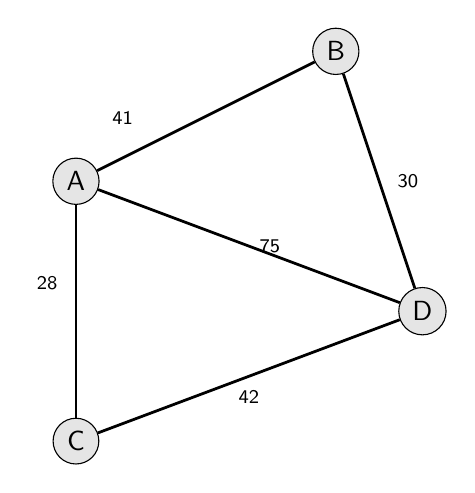
\begin{tikzpicture}[scale=1.1]
\tikzset{every node/.style={font=\sffamily}}
% Nodes (positions can be adjusted for a similar look)
\node[circle,draw,fill=black!10,inner sep=2.5pt] (A) at (0,1.5) {A};
\node[circle,draw,fill=black!10,inner sep=2.5pt] (B) at (3,3) {B};
\node[circle,draw,fill=black!10,inner sep=2.5pt] (D) at (4,0) {D};
\node[circle,draw,fill=black!10,inner sep=2.5pt] (C) at (0,-1.5) {C};

% Edges with weights
\draw[line width=1pt] (A) -- node[above left=0.1cm, near start] {\scriptsize 41} (B);
\draw[line width=1pt] (B) -- node[right=0.1cm, midway] {\scriptsize 30} (D);
\draw[line width=1pt] (A) -- node[right, midway] {\scriptsize 75} (D);
\draw[line width=1pt] (A) -- node[below left=0.1cm, near start] {\scriptsize 28} (C);
\draw[line width=1pt] (C) -- node[below=0.05cm, midway] {\scriptsize 42} (D);

% Optional: dots for emphasis
%\fill (A) circle (1.1pt);
%\fill (B) circle (1.1pt);
%\fill (C) circle (1.1pt);
%\fill (D) circle (1.1pt);

\end{tikzpicture}
\end{center}

\end{document}
